\chapter{Conclusiones y trabajos futuros}

\section{Conclusiones}

Vamos a separar este capítulo en partes entre las cuales están la revision del alcance de los objetivos donde se discutirá la medida en los que se han cumplido estos, valoración personal sobre el trabajo realizado, cumplimiento de los principios del desarrollo sostenible, futuro empresarial del software y los trabajos futuros para ampliar el alcance del software desarrollado.

\section{Objetivos}

Los objetivos perseguidos en este trabajo han sido los previamente mencionados en la sección objetivos en la introducción, los cuales son:
\begin{itemize}
	\item Analizar algunas apps del mercado, así como sus características, qué ofrecen, su costo para el usuario y las valoraciones de los usuarios finales, para aclarar qué es lo que buscan los usuarios en este tipo de apps y considerar esas necesidades en el software a desarrollar.
	\item Investigar sobre qué herramientas usar para la implementación de la base de datos, backend, frontend, y técnicas y metodologías para dar un desarrollo de calidad al software y para ayudar a la sostenibilidad del sistema en el tiempo.
	\item Conocer y aprender a usar herramientas actuales y punteras para el desarrollo de aplicaciones móviles. 
	\item Desarrollar una aplicación multiplataforma que cubra todos los requisitos necesarios para dar soporte a la planificación y realización de entrenamientos y monitorización de rutinas de ejercicio físico. 
	\item Tratar de obtener un software lo más accesible posible.
\end{itemize}

Analizando cada objetivo individualmente:
\begin{enumerate}
	\item \textbf{Analizar algunas apps del mercado, así como sus características, qué ofrecen, su costo para el usuario y las valoraciones de los usuarios finales, para aclarar qué es lo que buscan los usuarios en este tipo de apps y considerar esas necesidades en el software a desarrollar}: en el capítulo 2 se trata el estado el arte, en el cuál se mencionan las apps examinadas y las ventajas/desventajas de cada una respecto al software desarrollado, por tanto este objetivo se da por cumplido.
	\item \textbf{Investigar sobre qué herramientas usar para la implementación de la base de datos, backend, frontend, y técnicas y metodologías para dar un desarrollo de calidad al software y para ayudar a la sostenibilidad del sistema en el tiempo}: durante la realización del capítulo de estado del arte se examinaron distintas herramientas a usar, evidentemente no se iban a usar todas las examinadas pero aún sin haber puesto en práctica alguna de las tecnologías examinadas se aprendió sobre su uso y situaciones en las que emplearlas. Sobre las tecnologías previamente ya conocidas, se profundizó más sobre su uso. Este objetivo también se ha cumplido.
	\item \textbf{Conocer y aprender a usar herramientas actuales y punteras para el desarrollo de aplicaciones móviles}: este apartado esta muy relacionado con el anterior. Sin duda lo que más se ha mejorado es el trabajo con la metodología SCRUM, gracias a que durante el desarrollo se ha usado la herramienta web Jira de Atlassian para tener apoyo en la planificación y seguimiento de iteraciones, se ha mejorado su entendimiento y refinado conceptos que se creían aprendidos. cabe resaltar la soltura desarrollada con el framework Express.js(Node.js), que permitió el desarrollo de una API de forma rápida y fácil. Se cumplió este objetivo.
	\item \textbf{Desarrollar una aplicación multiplataforma que cubra todos los requisitos necesarios para dar soporte a la planificación y realización de entrenamientos y monitorización de rutinas de ejercicio físico}: Se ha cumplido este objetivo, pues se ha desarrollado una aplicacion con un entorno de programación multiplataforma cubriendo prácticamente todas las funcionalidades planificadas. Han quedado sin desarrollar pocas funcionalidades a las que se dio menor prioridad y que quedarán como trabajos futuros  a realizar.
	\item \textbf{Tratar de obtener un software lo más accesible posible}: No se ha cumplido por completo, dado que habría que mejorar algunos aspectos como tener iconos significativos en todos los elementos seleccionables. No obstante, el usuario siempre controla el flujo de la app, el software nunca hace cambios bruscos de pantalla ,ni presenta destellos molestos además de poseer una paleta de colores que relaja al usuario.
\end{enumerate}

\section{Valoración personal}

Hacer este TFG ha supuesto un gran desafio tanto académico como personal. Me he enfrentado a problemas de desarrollo y diseño reales de aplicaciones completas, como pueden ser fallos en la planificación, decidir si descartar una funcionalidad o no. Lo que más se ha refinado es la forma de trabajar usando metodología ágil SCRUM, que ya se había trabajado previamente en el grado, pero me ha permitido profundizar aún más, mejorando mi capacidad de organización, priorización de tareas y adaptación a cambios. Además, he tomado conciencia de la importancia del diseño centrado en el usuario y la accesibilidad.

También me ha ayudado a desarrollar mi comunicación, tanto creando esta documentación técnica como expresando datos técnicos a usuarios en la propia app. Además se mejoró también la comunicación personal en las diferentes reuniones ya sea explicando dudas e ideas sobre la app y su desarrollo.

\section{Objetivos de desarrollo sostenible}

La integración de principios de desarrollo sostenible en la creación y evolución de la app no solo garantiza su viabilidad a largo plazo, también asegura que el impacto de la aplicación sea positivo tanto para los usuarios como para el entorno. A medida que el mercado y las tecnologías evolucionen, la app puede adaptarse y crecer.

\begin{figure}[H]
    \centering
    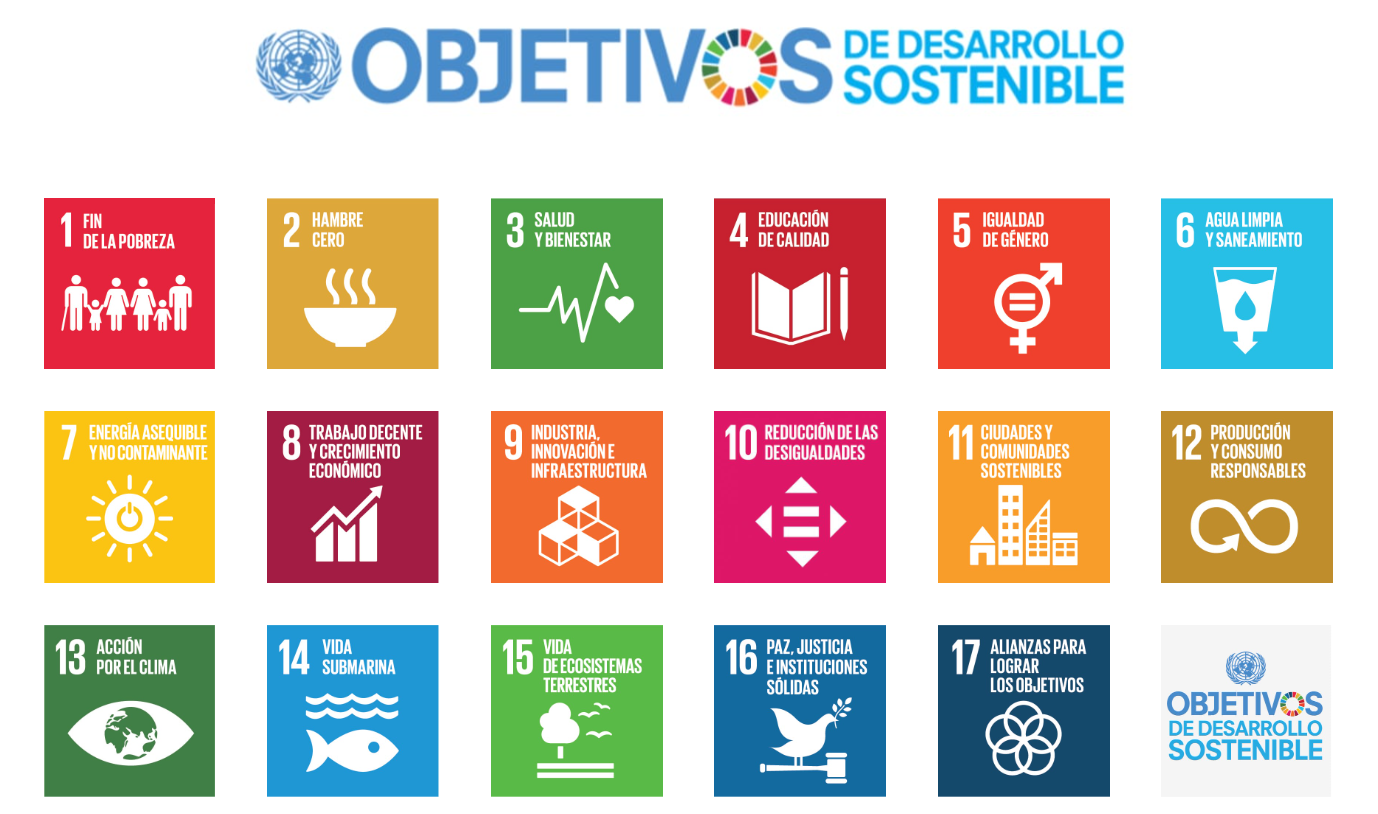
\includegraphics[width=0.8\textwidth]{fotos/2030.png}
    \caption{Objetivos desarrollo sostenible}
    \label{fig:2030}
\end{figure}

La app creada cubre por tanto los siguientes ODS:
\begin{itemize}
	\item \textbf{Número 3: Salud y bienestar}, la aplicación hace que el usuario respete los tiempos de descanso evitando lesiones
	\item \textbf{Número 10: Reducción de desigualdades}, se cumple al haber realizado una app teniendo en cuenta que sea accesible y tenga un diseño inclusivo
\end{itemize}

\section{Futuro empresarial}

La intención no es convertirlo en un negocio por ahora, creemos que sería necesario añadir alguna funcionalidad para hacer sentir al usuario que merece la pena pagar una cantidad por usar la app, no obstante se presentan algunas formas de monetizar la app:

\begin{itemize}
	\item Dar una versión gratuita con funcionalidades limitadas y otra versión de pago que de funcionalidades más completas y refinadas
	\item Se podría limitar el número de elementos en la nube por usuario y si este quisiese ampliar dicho número que pagué por esa ampliación 
	\item Hacer que la app la puedan usar gimnasios permitiendo que los mismos suban rutinas como si fueran un usuario más y ellos serían los que paguen por estar en la nube
\end{itemize}

\section{Trabajos futuros}

lgunas funcionalidades planteadas en el backlog se han quedado sin realizar, en concreto las relacionadas con tratamiento de datos de ejercicio físico, smartwatch e IA. Pasamos a describir cuáles son y cómo se abodarían:
\hspace{0.5cm}

\textbf{Tratamiento de datos del usuario}
\begin{itemize}
		\item[\textbf{SCRUM-10}] Valorar el entrenamiento en base a la marca actual y la meta del usuario
		\item[\textbf{SCRUM-12}] Medir pulso en reposo y compararlo con datos de ejercicios
		\item[\textbf{SCRUM-19}] Resumir datos
		\item[\textbf{SCRUM-22}] Interpretar constantes
\end{itemize}

\hspace{0.5cm}

Se estuvo investigando sobre la forma de averiguar en base a algunas constantes medidas del usuario si un entrenamiento esta siendo fructifero. Por ejemplo, si medimos el pulso de un usuario en reposo, es decir sin entrenar podemos detectar si se ha recuperado de su anterior entrenamiento.

\hspace{0.5cm}

\textbf{Relacionadas con la IA}
\begin{itemize}
		\item[\textbf{SCRUM-17}] Conectar con la IA para iniciar diálogo
\end{itemize}

\hspace{0.5cm}

Se investigó sobre ciertas IA entrenadas para deporte pero no se encontró mucha información. La mejor opción sería entonces entrenar una imagen de Llama con información de ciencias del deporte para despues usarla. 

\hspace{0.5cm}

\textbf{Relacionadas con el smartwatch}
\begin{itemize}
  	\item[\textbf{SCRUM-11}] Monitorizar pulso en tiempo real
	\item[\textbf{SCRUM-13}] Avisar de anomalías en el pulso de forma suave
	\item[\textbf{SCRUM-14}] Obtener calorías quemadas
	\item[\textbf{SCRUM-15}] Comprobar el equilibrio nervioso del usuario
	\item[\textbf{SCRUM-21}] Medir SpO2
\end{itemize}

\hspace{0.5cm}

Se encontraron librerías que permitían obtener estos datos de un reloj inteligente conectado por bluetooth de forma fácil. Se usaría la librería de flutter 'wear' que permite obtener todas las métricas disponibles de un reloj inteligente.

Todas estas se podrían implementar para versiones futuras. También se podrían añadir videos explicativos a los ejercicios, añadir más parámetros de medición a los ejercicios, etc.